% Options for packages loaded elsewhere
\PassOptionsToPackage{unicode}{hyperref}
\PassOptionsToPackage{hyphens}{url}
\PassOptionsToPackage{dvipsnames,svgnames,x11names}{xcolor}
%
\documentclass[
]{article}
\usepackage{amsmath,amssymb}
\usepackage{iftex}
\ifPDFTeX
  \usepackage[T1]{fontenc}
  \usepackage[utf8]{inputenc}
  \usepackage{textcomp} % provide euro and other symbols
\else % if luatex or xetex
  \usepackage{unicode-math} % this also loads fontspec
  \defaultfontfeatures{Scale=MatchLowercase}
  \defaultfontfeatures[\rmfamily]{Ligatures=TeX,Scale=1}
\fi
\usepackage{lmodern}
\ifPDFTeX\else
  % xetex/luatex font selection
\fi
% Use upquote if available, for straight quotes in verbatim environments
\IfFileExists{upquote.sty}{\usepackage{upquote}}{}
\IfFileExists{microtype.sty}{% use microtype if available
  \usepackage[]{microtype}
  \UseMicrotypeSet[protrusion]{basicmath} % disable protrusion for tt fonts
}{}
\makeatletter
\@ifundefined{KOMAClassName}{% if non-KOMA class
  \IfFileExists{parskip.sty}{%
    \usepackage{parskip}
  }{% else
    \setlength{\parindent}{0pt}
    \setlength{\parskip}{6pt plus 2pt minus 1pt}}
}{% if KOMA class
  \KOMAoptions{parskip=half}}
\makeatother
\usepackage{xcolor}
\usepackage[margin=1in]{geometry}
\usepackage{longtable,booktabs,array}
\usepackage{calc} % for calculating minipage widths
% Correct order of tables after \paragraph or \subparagraph
\usepackage{etoolbox}
\makeatletter
\patchcmd\longtable{\par}{\if@noskipsec\mbox{}\fi\par}{}{}
\makeatother
% Allow footnotes in longtable head/foot
\IfFileExists{footnotehyper.sty}{\usepackage{footnotehyper}}{\usepackage{footnote}}
\makesavenoteenv{longtable}
\usepackage{graphicx}
\makeatletter
\def\maxwidth{\ifdim\Gin@nat@width>\linewidth\linewidth\else\Gin@nat@width\fi}
\def\maxheight{\ifdim\Gin@nat@height>\textheight\textheight\else\Gin@nat@height\fi}
\makeatother
% Scale images if necessary, so that they will not overflow the page
% margins by default, and it is still possible to overwrite the defaults
% using explicit options in \includegraphics[width, height, ...]{}
\setkeys{Gin}{width=\maxwidth,height=\maxheight,keepaspectratio}
% Set default figure placement to htbp
\makeatletter
\def\fps@figure{htbp}
\makeatother
\setlength{\emergencystretch}{3em} % prevent overfull lines
\providecommand{\tightlist}{%
  \setlength{\itemsep}{0pt}\setlength{\parskip}{0pt}}
\setcounter{secnumdepth}{5}
\newlength{\cslhangindent}
\setlength{\cslhangindent}{1.5em}
\newlength{\csllabelwidth}
\setlength{\csllabelwidth}{3em}
\newlength{\cslentryspacingunit} % times entry-spacing
\setlength{\cslentryspacingunit}{\parskip}
\newenvironment{CSLReferences}[2] % #1 hanging-ident, #2 entry spacing
 {% don't indent paragraphs
  \setlength{\parindent}{0pt}
  % turn on hanging indent if param 1 is 1
  \ifodd #1
  \let\oldpar\par
  \def\par{\hangindent=\cslhangindent\oldpar}
  \fi
  % set entry spacing
  \setlength{\parskip}{#2\cslentryspacingunit}
 }%
 {}
\usepackage{calc}
\newcommand{\CSLBlock}[1]{#1\hfill\break}
\newcommand{\CSLLeftMargin}[1]{\parbox[t]{\csllabelwidth}{#1}}
\newcommand{\CSLRightInline}[1]{\parbox[t]{\linewidth - \csllabelwidth}{#1}\break}
\newcommand{\CSLIndent}[1]{\hspace{\cslhangindent}#1}
\renewcommand{\topfraction}{0.9}
\renewcommand{\bottomfraction}{0.8}
\renewcommand{\textfraction}{0.1}
\renewcommand{\floatpagefraction}{0.8}
\ifLuaTeX
  \usepackage{selnolig}  % disable illegal ligatures
\fi
\IfFileExists{bookmark.sty}{\usepackage{bookmark}}{\usepackage{hyperref}}
\IfFileExists{xurl.sty}{\usepackage{xurl}}{} % add URL line breaks if available
\urlstyle{same}
\hypersetup{
  pdftitle={DiveLab: An Executable Framework for Teaching Control Engineering Through Scuba-Diving Dynamics},
  pdfauthor={Francesco Civardi},
  pdfkeywords={control education, Jupyter notebooks, buoyancy
dynamics, reproducible computation, positive feedback},
  colorlinks=true,
  linkcolor={Maroon},
  filecolor={Maroon},
  citecolor={Blue},
  urlcolor={Blue},
  pdfcreator={LaTeX via pandoc}}

\title{DiveLab: An Executable Framework for Teaching Control Engineering
Through Scuba-Diving Dynamics}
\author{Francesco Civardi}
\date{2026-09-30}

\begin{document}
\maketitle
\begin{abstract}
Control engineering is often taught through mathematically related
techniques whose physical continuity is left implicit. DiveLab instead
develops one causal system from hydrostatic pressure and gas compression
through buoyancy, vertical dynamics, estimation, feedback control, and
integrated resource models. The open-source framework pairs 18 textbook
chapters with 18 Google-Colab-compatible Jupyter notebooks and preserves
a common sign convention, state definition, and parameter set. We
formulate a local vertical plant and show that compression of flexible
gas creates a saddle equilibrium: the reference model has poles at
\(\pm0.1027\ \mathrm{s}^{-1}\). The same plant is then used for
observability, state estimation, pole placement, PID control, frequency
response, human-in-the-loop effects, breathing, gas consumption, and
inert-gas compartments. Execution of all notebooks in isolated Jupyter
kernels completed without Python exceptions and generated 64 figures.
Representative regression anchors include closed-loop poles at \(-0.6\)
and \(-0.9\
\mathrm{s}^{-1}\) and a reduction in integral absolute error from 177.47
to 5.17 m s in the specified anti-windup experiment. DiveLab is an
educational modeling framework, not an operational dive-planning or
safety system. No learning-outcome claim is made without a future
classroom study.
\end{abstract}

\hypertarget{introduction}{%
\section{Introduction}\label{introduction}}

Engineering students commonly encounter hydrostatics, nonlinear
dynamics, linearization, estimation, and feedback as separate topics.
The mathematical links are apparent to an experienced engineer but can
remain hidden to a learner when the physical system changes in every
chapter. DiveLab explores a different curriculum design: retain one
physical narrative and progressively increase the fidelity and
analytical viewpoint of its model. Its technical sequence draws on
standard control-system concepts
(\protect\hyperlink{ref-ogata2010}{Ogata 2010};
\protect\hyperlink{ref-astrom2008}{Åström and Murray 2008}), while its
executable form follows the literate, reproducible-workflow role of
Jupyter notebooks (\protect\hyperlink{ref-kluyver2016}{Kluyver et al.
2016}; \protect\hyperlink{ref-granger2021}{Granger and Pérez 2021}).

Scuba-diving dynamics provide a compact organizing example. Ambient
pressure changes with depth; flexible gas volumes change with pressure;
those volume changes modify buoyancy; buoyancy modifies vertical motion;
and motion feeds the pressure change back into the loop. Sensing,
estimation, actuation, human decisions, breathing, gas resources, and
inert-gas states extend this causal chain. The result is a system model
that grows with the curriculum rather than a collection of unrelated
demonstrations.

The paper makes three contributions:

\begin{enumerate}
\def\labelenumi{\arabic{enumi}.}
\tightlist
\item
  a pedagogical formulation of a standard vertical plant exposing the
  positive-feedback mechanism near neutral buoyancy;
\item
  an executable architecture in which 18 chapters and notebooks share
  notation, parameters, and causal continuity; and
\item
  a reproducible, repository-level validation of the full notebook
  sequence, including numerical anchors and explicit evidence and safety
  boundaries.
\end{enumerate}

This is a framework and artifact paper. It asks whether a physically
coherent example can be represented consistently across a
control-engineering sequence and whether the resulting computational
artifact executes reproducibly. It does not ask whether DiveLab improves
student learning; that question requires a separate empirical study.

\hypertarget{related-work-and-design-gap}{%
\section{Related work and design
gap}\label{related-work-and-design-gap}}

Notebook-centered teaching has been used to combine exposition, code,
and results in engineering curricula. Engineers Code organized reusable
open learning modules as Jupyter lessons
(\protect\hyperlink{ref-barba2020}{Barba 2020}), and
chemical-engineering work has used notebooks for problem generation and
classroom exposition (\protect\hyperlink{ref-dominguez2021}{Domínguez et
al. 2021}). More generally, computational notebooks support narratives
in which equations, code, data, and figures remain adjacent
(\protect\hyperlink{ref-granger2021}{Granger and Pérez 2021}). Their
reproducibility is not automatic, however: execution order, hidden
state, dependency drift, and incomplete environments can undermine an
apparently self-contained artifact
(\protect\hyperlink{ref-samuel2024}{Samuel and Mietchen 2024}). DiveLab
therefore treats whole-curriculum execution as a tested property rather
than an assumed benefit of the file format.

Scuba buoyancy has also been modeled for engineering purposes. Valenko
et al. developed and experimentally compared a detailed nonlinear diver,
buoyancy- compensator, and pneumatic-valve model
(\protect\hyperlink{ref-valenko2016}{Valenko et al. 2016}). Subsequent
work has used such dynamics in automatic buoyancy controllers, including
fuzzy-control designs (\protect\hyperlink{ref-muskinja2023}{Muškinja,
Rižnar, and Golob 2023}). DiveLab has a different purpose and
deliberately lower model fidelity: it uses the minimum model needed to
reveal a causal feedback loop and then revisits that same plant through
successive control concepts. The detailed physical literature
establishes that buoyancy control is a legitimate dynamic- systems
problem; DiveLab contributes the vertically integrated, executable
curriculum around it.

A recent preprint explicitly analyzes a diver as a delayed PD regulator
of a compressible-buoyancy saddle and studies delay-induced oscillation
and saturation (\protect\hyperlink{ref-herho2026}{Herho et al. 2026}).
That work reinforces the distinction between DiveLab's curriculum
contribution and dynamical analysis of diver control. DiveLab does not
claim priority for the physical instability mechanism or for delayed
diver feedback.

The design gap is thus not the absence of notebook-based instruction or
diver models separately. It is the absence, to our knowledge, of an
openly executable control curriculum that follows this particular
human-in-the-loop plant from first principles to a capstone while
preserving a traceable set of assumptions and numerical regression
anchors.

\hypertarget{mathematical-framework}{%
\section{Mathematical framework}\label{mathematical-framework}}

\hypertarget{coordinates-pressure-and-gas-compression}{%
\subsection{Coordinates, pressure, and gas
compression}\label{coordinates-pressure-and-gas-compression}}

Let depth \(z\) be positive downward and vertical velocity \(v\) be
positive upward, so \(\dot z=-v\). This mixed convention is intentional:
depth matches diving practice, while positive force and velocity remain
upward. With water density \(\rho\), gravitational acceleration \(g\),
and surface absolute pressure \(P_0\),

\[
P(z)=P_0+\rho g z.
\]

Assuming isothermal ideal-gas compression for a flexible volume \(V_g\),
with surface-equivalent volume \(V_{g0}\),

\[
V_g(z)=V_{g0}\frac{P_0}{P(z)}.
\]

The nonlinearity is strongest near the surface: equal depth changes do
not cause equal fractional volume changes. Figure 1 is generated by
Notebook 02 from the same pressure function used downstream.

\begin{figure}
\hypertarget{fig-boyle}{%
\centering
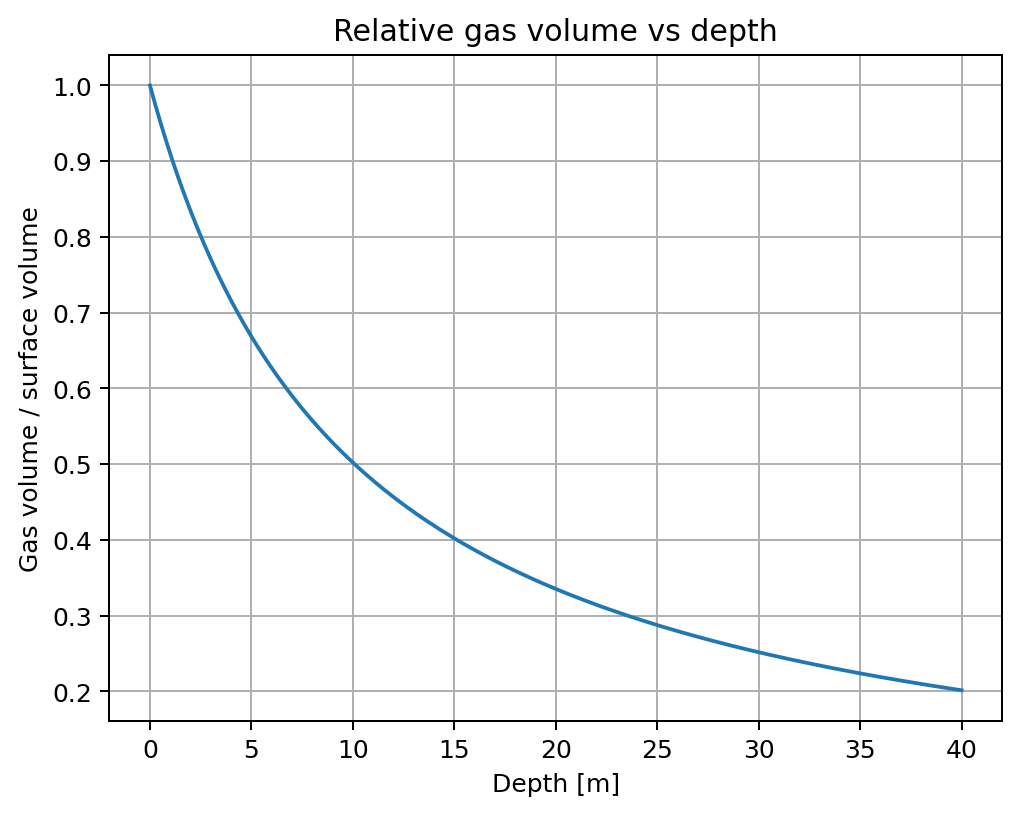
\includegraphics[width=0.75\textwidth,height=\textheight]{generated/boyle-volume-depth.png}
\caption{Flexible-gas volume under the isothermal Boyle-law
model.}\label{fig-boyle}
}
\end{figure}

\hypertarget{forces-and-nonlinear-state-model}{%
\subsection{Forces and nonlinear state
model}\label{forces-and-nonlinear-state-model}}

Let \(m\) denote total mass, \(V_f\) the approximately fixed displaced
volume, \(F_D(v)\) hydrodynamic drag, and \(u\) an abstract upward
control force. Archimedes' principle gives

\[
F_B(z)=\rho g\left[V_f+V_g(z)\right].
\]

The vertical dynamics are

\[
\dot z=-v, \qquad
m\dot v=F_B(z)-mg+F_D(v)+u.
\]

The notebooks use the sign-opposing quadratic drag law

\[
F_D(v)=-c_D v|v|,
\]

which is continuous but has zero derivative at \(v=0\). The input \(u\)
is an educational abstraction. A real buoyancy compensator changes gas
volume through valve dynamics rather than applying force
instantaneously; omitting those dynamics keeps the early control
examples interpretable and is revisited as a limitation.

\hypertarget{equilibrium-and-local-instability}{%
\subsection{Equilibrium and local
instability}\label{equilibrium-and-local-instability}}

At a neutral equilibrium \((z_e,0)\) with \(u=0\), \(F_B(z_e)=mg\).
Define

\[
k_B=\left.\frac{dF_B}{dz}\right|_{z_e}
=-\rho^2g^2V_{g0}\frac{P_0}{(P_0+\rho g z_e)^2}<0.
\]

With perturbation state \(x=[\delta z,\delta v]^T\), and ignoring the
quadratic drag term in the infinitesimal linearization,

\[
\dot x=Ax+B\delta u,\qquad
A=\begin{bmatrix}0&-1\\k_B/m&0\end{bmatrix},\quad
B=\begin{bmatrix}0\\1/m\end{bmatrix}.
\]

The characteristic equation is

\[
\lambda^2+\frac{k_B}{m}=0,
\]

so \(k_B/m<0\) gives two real poles with opposite signs. This is a
saddle, not an oscillatory neutral mode. In physical terms, a small
downward displacement compresses flexible gas, reduces buoyancy, and
promotes further descent; an upward displacement expands it and promotes
further ascent. The feedback is positive around the chosen equilibrium.

For the reference values \(m=85\) kg,
\(\rho=1025\ \mathrm{kg\,m^{-3}}\), \(z_e=20\) m,
\(g=9.80665\ \mathrm{m\,s^{-2}}\), \(P_0=101325\) Pa, and
\(V_{g0}=0.008\ \mathrm{m^3}\) (8 L surface-equivalent gas), the neutral
fixed volume is \(V_f=m/\rho-V_g(z_e)=0.080246\ \mathrm{m^3}\).
Numerical and analytic derivatives agree at
\(k_B=-0.895866\ \mathrm{N\,m^{-1}}\). The poles are
\(\lambda=\pm0.102663\ \mathrm{s^{-1}}\), giving an unstable-mode
e-folding time of 9.741 s. Figure 2 displays the local nonlinear vector
field and the linear eigendirections.

\begin{figure}
\hypertarget{fig-saddle}{%
\centering
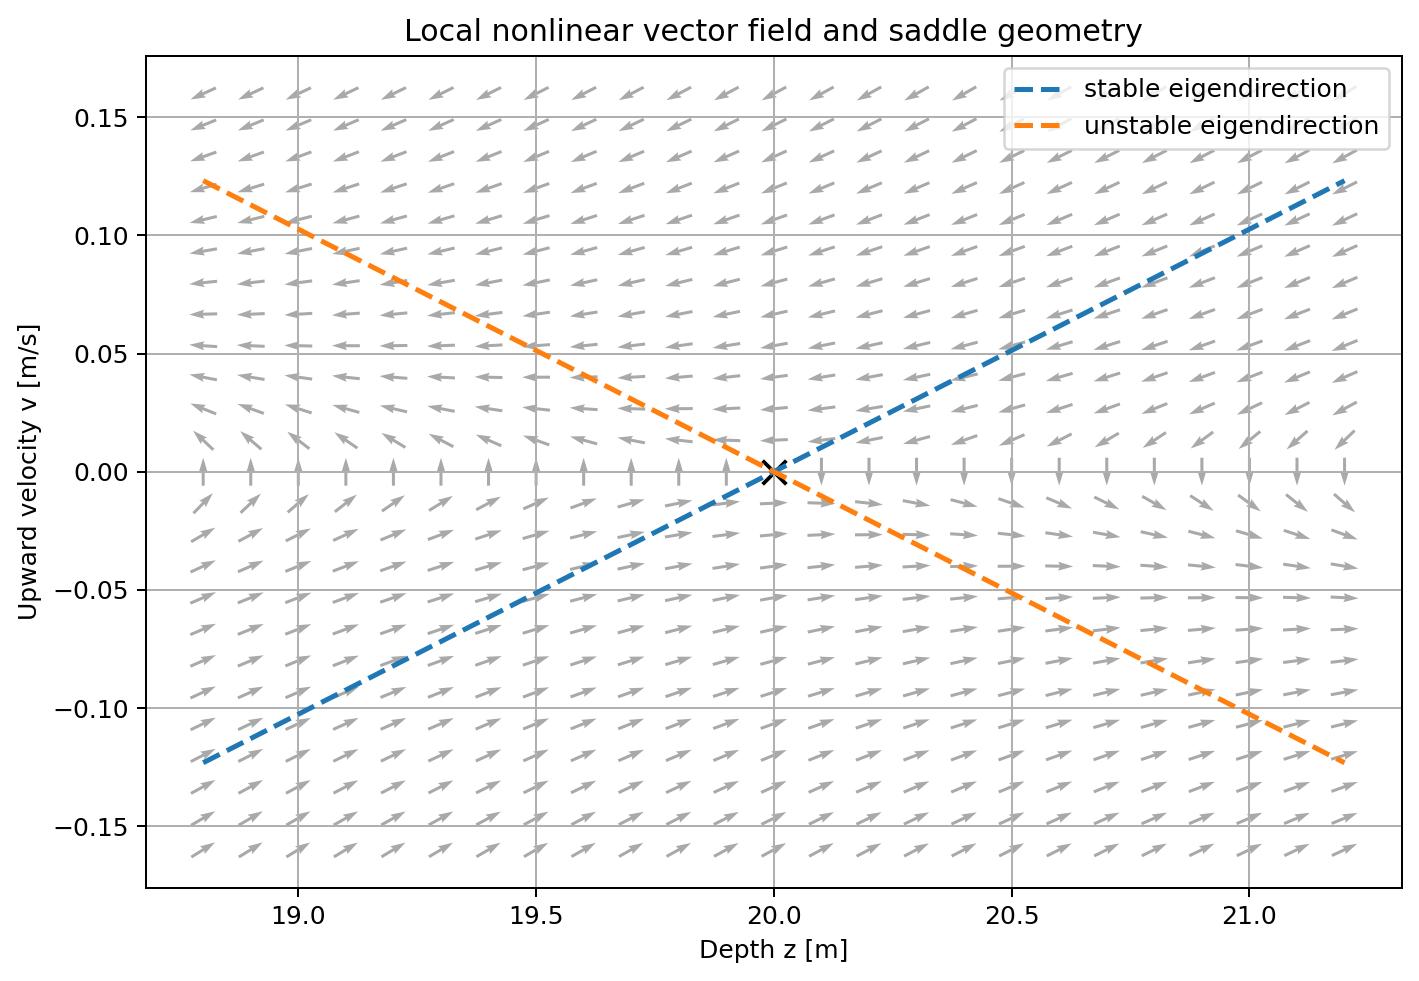
\includegraphics[width=0.85\textwidth,height=\textheight]{generated/saddle-vector-field.png}
\caption{Local nonlinear vector field around neutral buoyancy. The
dashed lines are the stable and unstable eigendirections of the
linearization.}\label{fig-saddle}
}
\end{figure}

\hypertarget{executable-curriculum-architecture}{%
\section{Executable curriculum
architecture}\label{executable-curriculum-architecture}}

\hypertarget{progression-and-traceability}{%
\subsection{Progression and
traceability}\label{progression-and-traceability}}

The curriculum follows four stages (Table 1). Each canonical chapter has
a same-numbered notebook. Every notebook can run independently in Google
Colab, while later notebooks reuse the earlier coordinate convention,
pressure law, plant structure, and reference parameters.

\begin{table}[htbp]
\centering
\caption{Curriculum progression and its causal hand-offs.}
\small
\begin{tabular}{p{0.14\linewidth}p{0.10\linewidth}p{0.35\linewidth}p{0.25\linewidth}}
\toprule
Stage & Notebooks & Primary ideas & Output carried forward \\
\midrule
Physical laws & 01--04 & Pressure, Boyle's law, Archimedes, vertical forces & Nonlinear buoyancy and force model \\
Dynamical systems & 05--09 & State space, equilibrium, linearization, observability, Kalman filtering, transfer functions & Local plant and estimators \\
Feedback & 10--14 & PD/PID, saturation, frequency response, human decisions, breathing disturbance & Controlled vertical response \\
Integrated systems & 15--18 & Gas consumption, dive-computer estimation, inert-gas states, capstone & Resource histories; separate local feedback \\
\bottomrule
\end{tabular}
\end{table}

The architecture separates explanation from experiment. Chapters derive
assumptions, equations, examples, and limitations. Notebooks expose
parameters, simulate alternatives, and produce numerical results. This
gives two linked views of the same material: a readable derivation and
an executable experiment.

\hypertarget{intended-learning-workflow}{%
\subsection{Intended learning
workflow}\label{intended-learning-workflow}}

Each module follows a recurring sequence:

\begin{enumerate}
\def\labelenumi{\arabic{enumi}.}
\tightlist
\item
  \textbf{Understand:} identify variables, signs, units, and causal
  direction.
\item
  \textbf{Model:} state assumptions and derive the governing relation.
\item
  \textbf{Simulate:} vary parameters and compare nonlinear and local
  models.
\item
  \textbf{Control or estimate:} introduce feedback, sensing,
  constraints, or state reconstruction only after the open-loop behavior
  is visible.
\item
  \textbf{Interpret:} distinguish mathematical results from operational
  diving conclusions.
\end{enumerate}

The repetition is deliberate. Learners encounter new control tools
without paying the cognitive cost of learning a new physical plant each
time. Conversely, the repeated plant exposes how a modeling decision
made early---such as treating actuation as force---propagates into later
conclusions.

\hypertarget{representative-computational-experiments}{%
\section{Representative computational
experiments}\label{representative-computational-experiments}}

\hypertarget{measurement-differentiation-and-state-estimation}{%
\subsection{Measurement, differentiation, and state
estimation}\label{measurement-differentiation-and-state-estimation}}

For a depth-only measurement \(y=Cx\) with \(C=[1\;0]\), the
observability matrix is

\[
\mathcal O=\begin{bmatrix}C\\CA\end{bmatrix}
=\begin{bmatrix}1&0\\0&-1\end{bmatrix},
\]

and therefore has rank two. Velocity can be reconstructed from the model
and a depth history. The notebook contrasts this with direct finite
differencing, which amplifies sample noise (Figure 3). Under the
specified synthetic noise and initial-error scenario, sampled at 0.01 s
with depth-noise standard deviation 0.02 m and random seed 42,
differentiation produces a velocity RMSE of 1.4356 m/s; a Luenberger
observer with requested poles at \(-0.7\) and \(-1.0\)
\(\mathrm{s^{-1}}\) produces 0.00078 m/s (Figure 4). Both errors are
evaluated over 5--20 s, excluding the initial transient. The true
initial state is \([0,0.05]^T\) and the observer starts at
\([0.30,-0.15]^T\), with depth in metres and velocity in metres per
second.

\begin{figure}
\hypertarget{fig-diff}{%
\centering
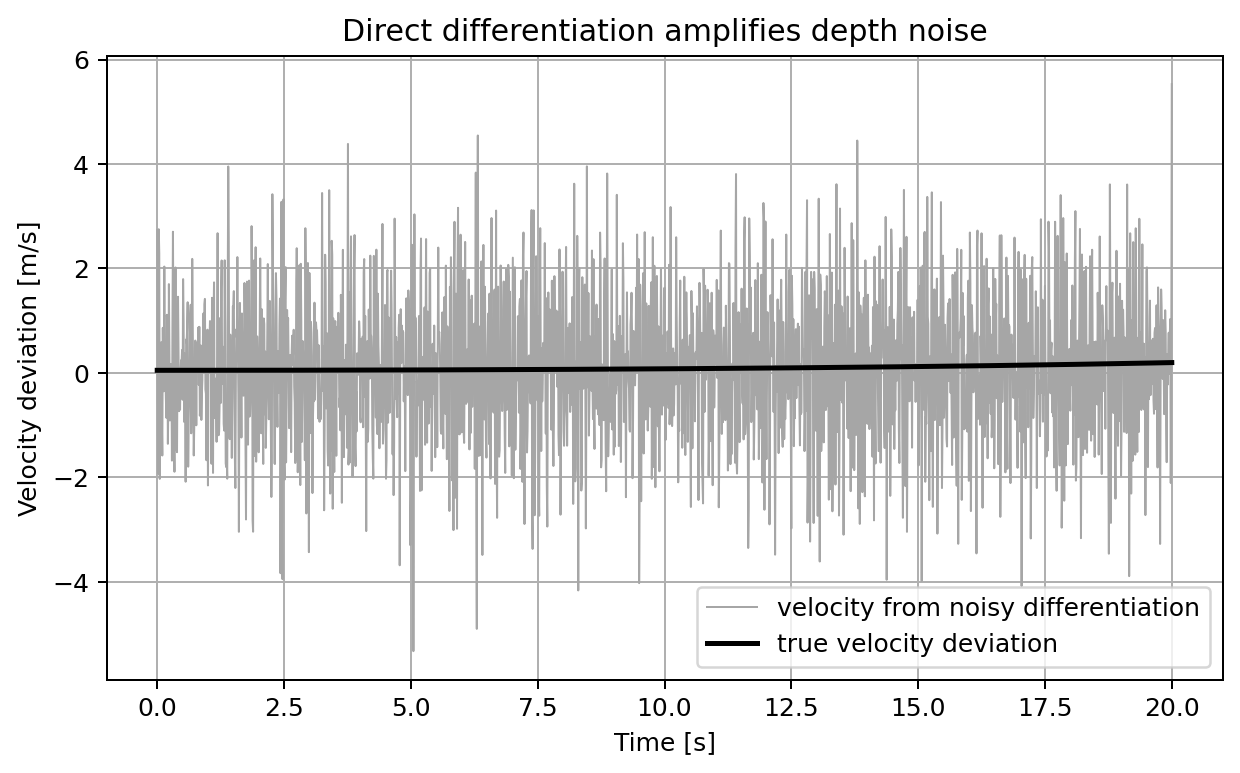
\includegraphics[width=0.78\textwidth,height=\textheight]{generated/differentiation-noise.png}
\caption{Direct numerical differentiation amplifies the synthetic
depth-measurement noise.}\label{fig-diff}
}
\end{figure}

\begin{figure}
\hypertarget{fig-observer}{%
\centering
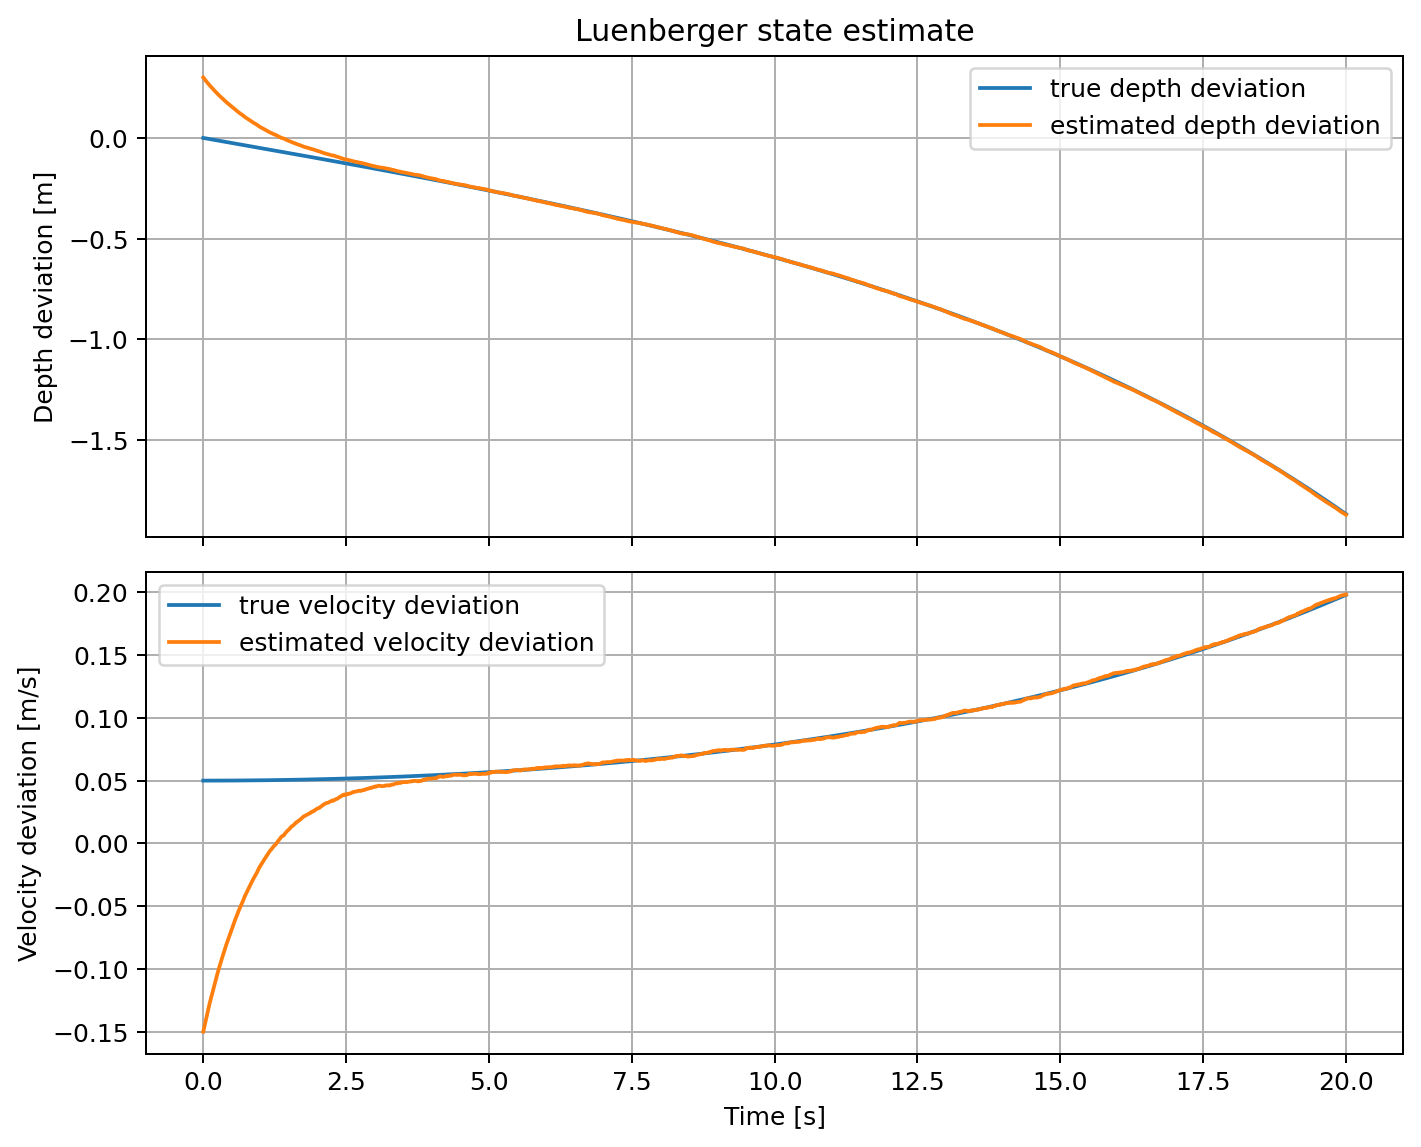
\includegraphics[width=0.82\textwidth,height=\textheight]{generated/observer-estimate.png}
\caption{Luenberger reconstruction of depth and velocity in the nominal
synthetic experiment.}\label{fig-observer}
}
\end{figure}

The magnitude of this difference must not be generalized to hardware. It
depends on a correct model, noise assumptions, initialization, and
sample rate. The experiment's instructional purpose is to make the
trade-off between a noisy algebraic operation and model-based dynamic
inference concrete. Notebook 08 then recasts estimation
probabilistically with a discrete Kalman filter, obtaining a velocity
RMSE of 0.01593 m/s in its separate stochastic scenario and exposing
sensitivity to \(Q\) and \(R\).

\hypertarget{state-feedback-and-integral-action}{%
\subsection{State feedback and integral
action}\label{state-feedback-and-integral-action}}

For full-state feedback \(\delta u=-Kx\), the notebook selects gains
that place the closed-loop poles at \(-0.6\) and
\(-0.9\ \mathrm{s^{-1}}\). Figure 5 compares the unstable open-loop
response with the regulated local model. The example demonstrates pole
placement, but its force command is not a claim about a realizable
buoyancy-compensator actuator.

\begin{figure}
\hypertarget{fig-feedback}{%
\centering
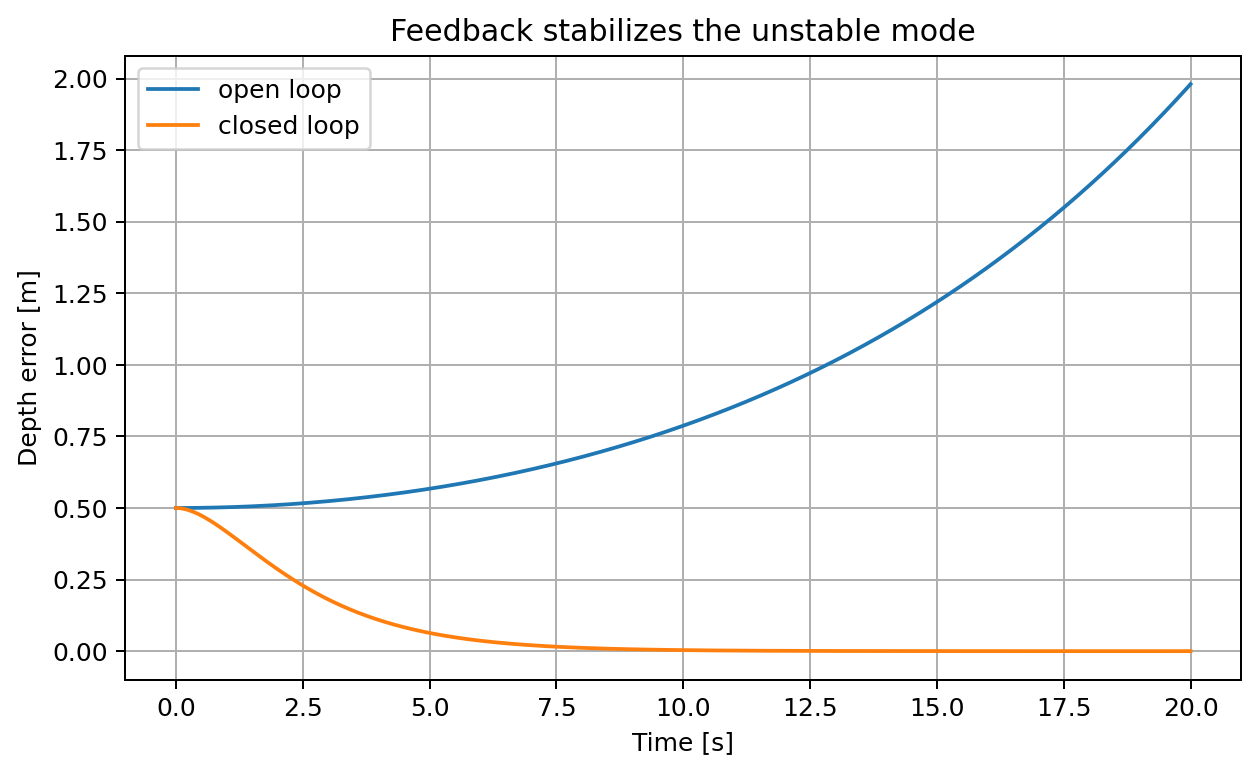
\includegraphics[width=0.75\textwidth,height=\textheight]{generated/open-closed-loop.png}
\caption{Open-loop growth and closed-loop regulation from the same
initial depth perturbation.}\label{fig-feedback}
}
\end{figure}

A constant disturbance produces the expected nonzero steady offset under
PD control: the analytical prediction and numerical result are both
\(-0.1089\) m in the stated test. Integral action removes this modeled
offset. It also creates a constraint problem when the actuator
saturates. In the deliberately severe Notebook 11 case, the gains are
\(K_p=150\) N/m, \(K_d=180\) N s/m, and \(K_i=60\) N/(m s). The initial
depth error is 2 m, the force limit is \(\pm35\) N, the disturbance is
zero, and the horizon is 35 s. The back-calculation coefficient is 0.02
m/N in \(\dot\eta=\delta z+K_{aw}(u-u_{raw})\). Integral absolute error
is 177.47 m s without protection and 5.17 m s with back-calculation
anti-windup. Figure 6 shows the internal integrator and requested force
diverging when saturation is ignored.

\begin{figure}
\hypertarget{fig-windup}{%
\centering
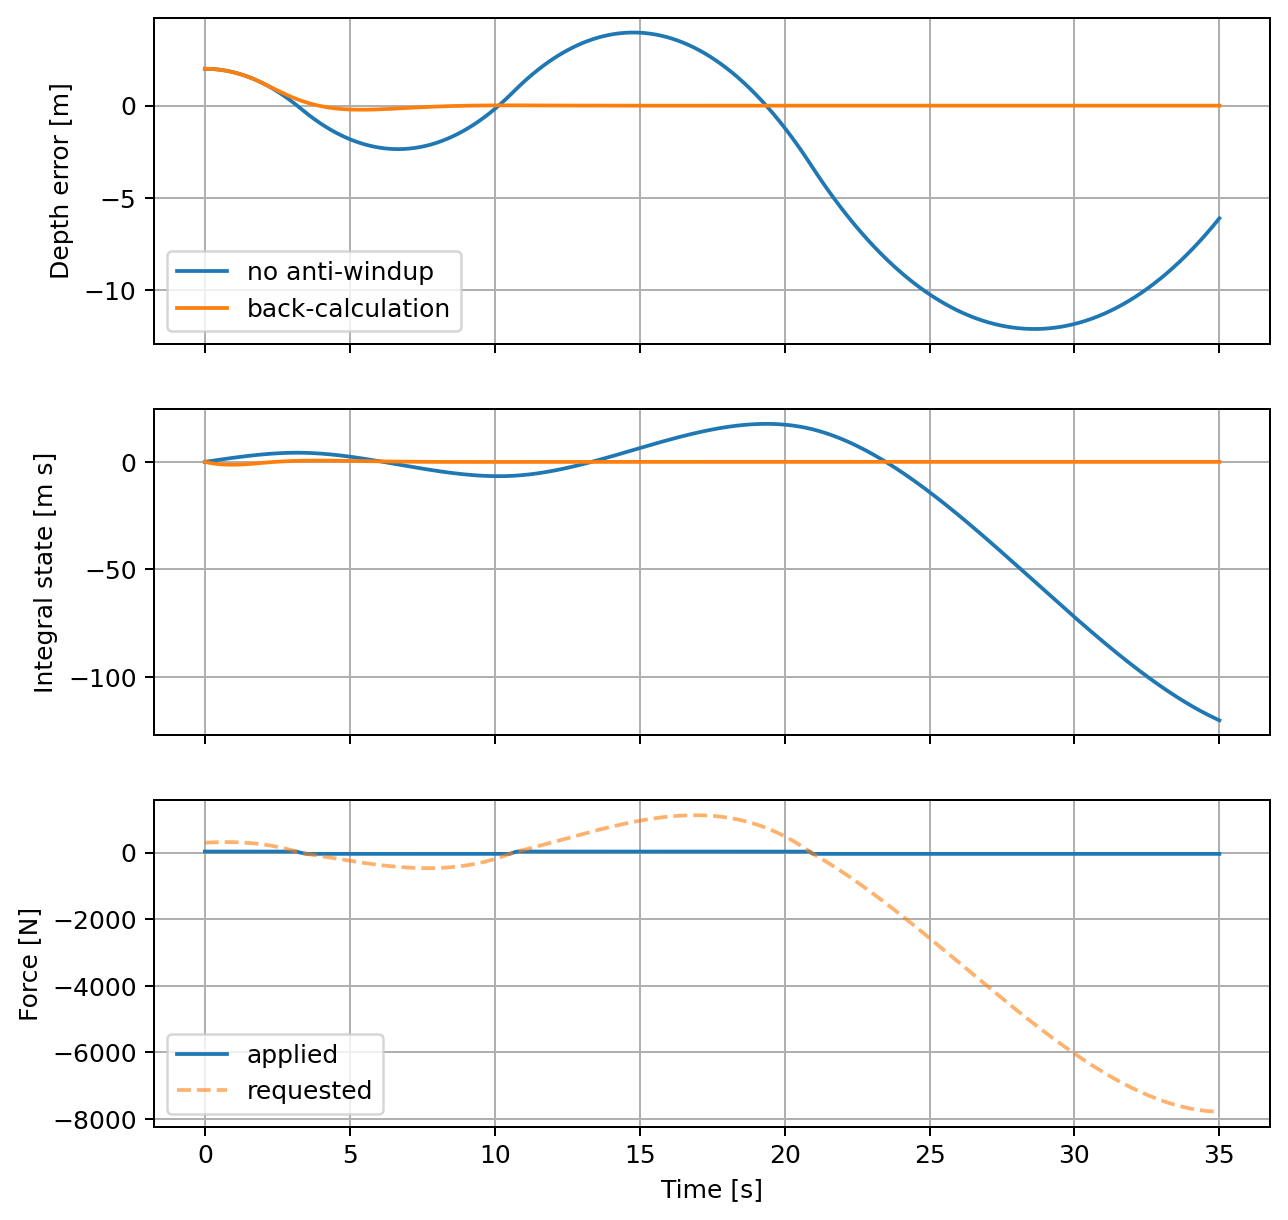
\includegraphics[width=0.85\textwidth,height=\textheight]{generated/anti-windup.png}
\caption{Saturation experiment contrasting an unprotected integrator
with back-calculation anti-windup.}\label{fig-windup}
}
\end{figure}

\hypertarget{frequency-domain-and-human-in-the-loop-views}{%
\subsection{Frequency-domain and human-in-the-loop
views}\label{frequency-domain-and-human-in-the-loop-views}}

The local closed-loop model has natural frequency 0.735 rad/s, damping
ratio 1.021, and an approximate \(-3\) dB bandwidth of 0.465 rad/s. The
frequency- response notebook uses those quantities to connect pole
placement to disturbance attenuation. Notebook 13 then replaces
continuous ideal feedback with sampled, delayed, quantized decisions.
Its particular ``predictive'' heuristic performs worse than the reactive
baseline (0.303 m versus 0.229 m RMS depth error), an important negative
result: adding anticipation is not intrinsically beneficial when its
model, timing, or gain is poor.

Breathing is introduced as a periodic buoyancy disturbance rather than
noise to be discarded. A 0.5 L volume change corresponds to
approximately 5.03 N in the reference seawater model. This allows the
same plant to link frequency response, disturbance rejection, and a
physiological action without claiming a complete respiratory model.

\hypertarget{integrated-capstone}{%
\subsection{Integrated capstone}\label{integrated-capstone}}

The final notebook contains two complementary experiments. In the first,
a prescribed depth history drives ambient-pressure calculation,
synthetic measurement, gas-use integration, and simplified parallel
inert-gas compartments with nominal half-times of 5, 20, 80, and 240
minutes. Figure 7 presents the coupled outputs on a common time base.
The second is a separate local feedback experiment around 18 m, with
poles at \(-0.35\) and \(-0.55\ \mathrm{s^{-1}}\) and a \(\pm12\) N
force limit. Its controlled depth is not fed back into the resource or
compartment histories shown in Figure 7. The capstone's main
contribution is architectural: quantities can be labeled as prescribed,
measured, derived, estimated, predicted, or controlled within one state
history.

\begin{figure}
\hypertarget{fig-capstone}{%
\centering
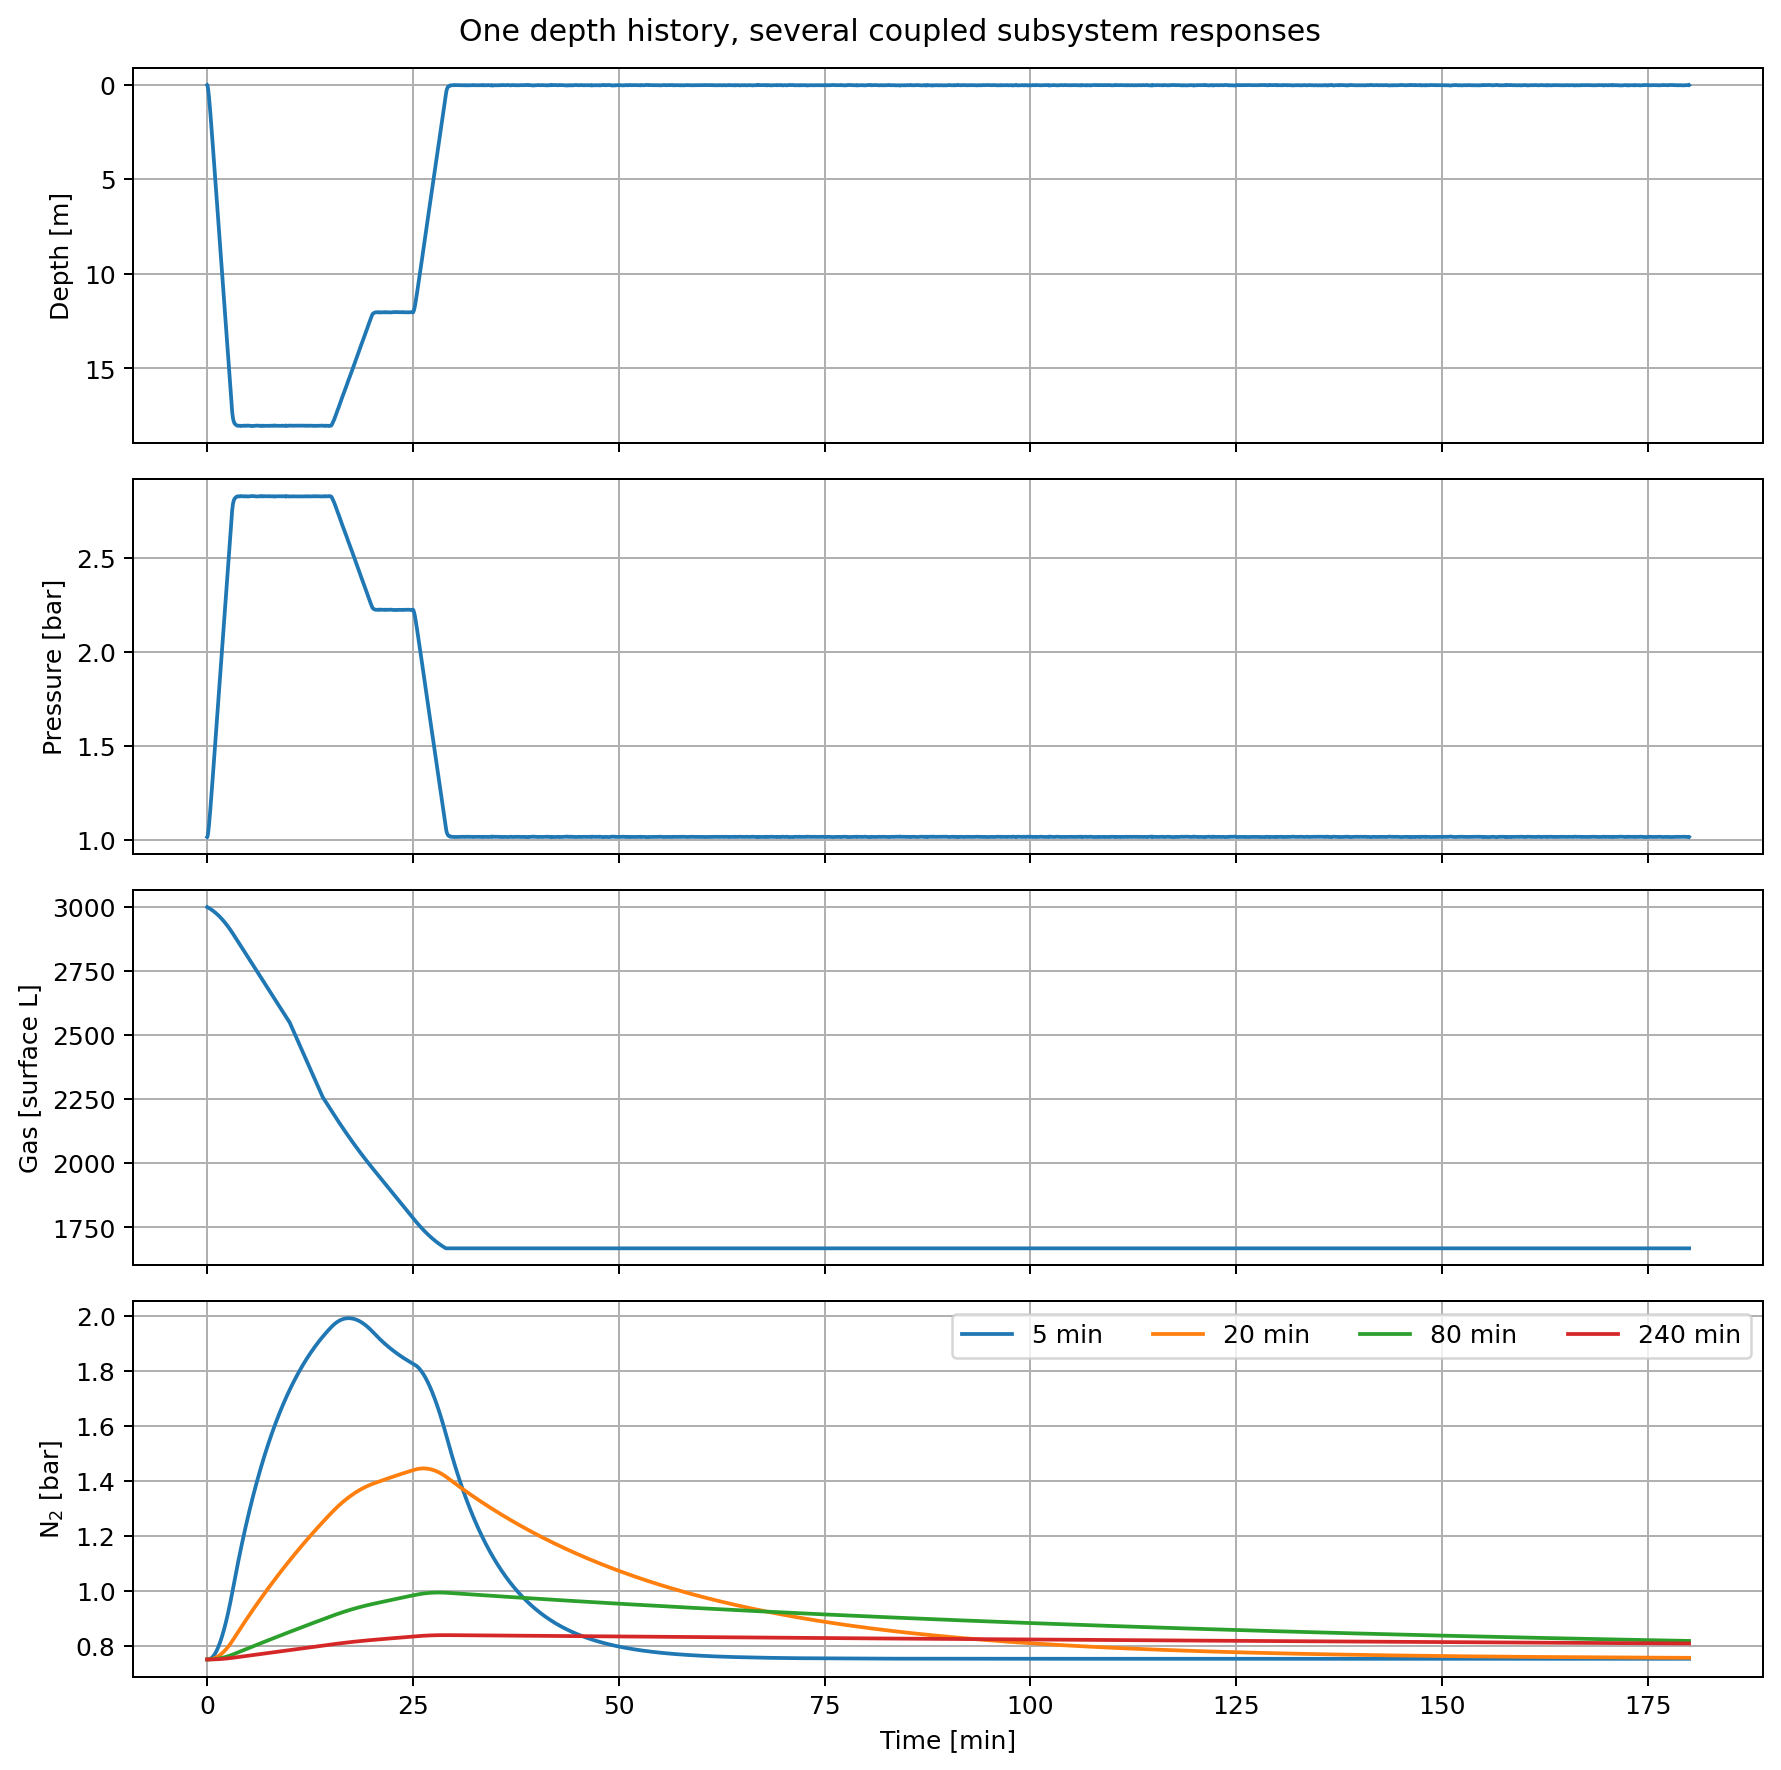
\includegraphics[width=0.95\textwidth,height=\textheight]{generated/capstone.png}
\caption{Capstone resource histories: prescribed depth drives estimated
pressure, gas use, and simplified inert-gas compartments. Local feedback
is evaluated separately.}\label{fig-capstone}
}
\end{figure}

The final depth error in the separate local experiment is \(-0.306\) m,
following a 5 N constant upward disturbance introduced at 12 s. It
agrees with the PD steady-state offset \(-5/[85(0.35)(0.55)]\) m; the
controller has no integral action. It is not a tracking error for the
prescribed piecewise dive profile. The resource histories and local
control experiment are complementary teaching examples rather than a
fully coupled dive simulation. Likewise, the compartment trajectories
demonstrate exponential memory; they do not produce decompression
ceilings or schedules.

\hypertarget{reproducibility-and-validation}{%
\section{Reproducibility and
validation}\label{reproducibility-and-validation}}

\hypertarget{artifact-structure}{%
\subsection{Artifact structure}\label{artifact-structure}}

The repository contains 18 chapter sources and 18 canonical notebooks.
Notebook imports are limited to NumPy, SciPy, and Matplotlib. The
release validator starts a fresh Jupyter kernel for each notebook using
\texttt{nbclient}, executes the original code cells in document order,
and captures Matplotlib figures after each cell. It uses the
non-interactive Agg backend so figure counting and export are explicit;
it is a kernel execution test, not a browser or Google Colab UI test. An
appended audit cell checks numerical anchors with explicit absolute
tolerances and zero relative tolerance. The validator requires exactly
18 notebooks, 64 figures, and all selected manuscript figures to be
present. The tested Python 3.12 dependency environment is recorded in
\texttt{paper/requirements-lock.txt}; the GitHub Actions workflow
repeats the kernel validation and compiles the standalone LaTeX source
on pushes and pull requests.

\hypertarget{validation-result-and-anchors}{%
\subsection{Validation result and
anchors}\label{validation-result-and-anchors}}

On Python 3.12 with NumPy 2.3.5, SciPy 1.17.0, and Matplotlib 3.10.8,
all 18 notebooks completed with zero Python exceptions and produced 64
figures. Table 2 records representative anchors selected across the
sequence.

\begin{longtable}[]{@{}lr@{}}
\caption{Representative numerical regression anchors.}\tabularnewline
\toprule\noalign{}
Experiment & Recomputed result \\
\midrule\noalign{}
\endfirsthead
\toprule\noalign{}
Experiment & Recomputed result \\
\midrule\noalign{}
\endhead
\bottomrule\noalign{}
\endlastfoot
Hydrostatic pressure gradient & 10051.82 Pa/m \\
Buoyancy derivative at 20 m & -0.895866 N/m \\
Open-loop poles & \(\pm0.102663\ \mathrm{s^{-1}}\) \\
Unstable e-folding time & 9.741 s \\
Observer velocity RMSE & 0.00078 m/s \\
Finite-difference velocity RMSE & 1.4356 m/s \\
Kalman-filter velocity RMSE & 0.01593 m/s \\
Designed closed-loop poles & -0.6, -0.9 \(\mathrm{s^{-1}}\) \\
Windup / anti-windup IAE & \(177.47 / 5.17\ \mathrm{m\cdot s}\) \\
\end{longtable}

These are deterministic or seeded computational checks, not measurements
of divers. The automated checks use absolute tolerances ranging from
\(10^{-10}\) for local closed-loop poles to \(10^{-4}\) m s for the
windup integral; rounded reported values are checked to their stated
precision. These tolerances detect regressions in the specified
numerical experiments, not physical model error. The LaTeX source
package compiles independently of Quarto-generated paths.

\hypertarget{evidence-safety-and-ethical-boundaries}{%
\section{Evidence, safety, and ethical
boundaries}\label{evidence-safety-and-ethical-boundaries}}

DiveLab currently supports claims about internal model consistency,
executable coverage, and curriculum architecture. It does not support a
claim that the approach improves learning outcomes because no learners
have yet been studied. A future evaluation should predefine the
participant population, prerequisites, learning objectives, pre/post
instruments, comparison condition, attrition handling, and statistical
analysis before data collection.

The models are educational. They do not generate operational
decompression limits, gas reserves, ascent schedules, medical
assessments, equipment certification, or permission to dive. Real diving
requires recognized training, appropriate supervision, suitable
equipment, medical assessment when indicated, and adherence to
established procedures. The computational use of a human diver as the
plant must not be interpreted as support for experimental automatic
buoyancy actuation on people.

\hypertarget{limitations-and-future-work}{%
\section{Limitations and future
work}\label{limitations-and-future-work}}

The capstone does not yet feed controlled motion into the full resource
and compartment history. The vertical model suppresses added
hydrodynamic mass, changing body geometry, equipment-specific gas
migration, actuator and valve dynamics, uncertain drag, currents, trim,
sensor faults, and individual physiology. Quadratic drag has zero local
derivative at the equilibrium, so damping visible in finite excursions
is absent from the infinitesimal linear plant. The control input is
force-like rather than a valve command. These choices aid instruction
but limit physical fidelity.

The physical and pedagogical validation remains incomplete. Successful
execution does not prove that every equation is physically accurate,
that every parameter is realistic, or that each pedagogical transition
is effective. Independent model review, uncertainty analysis and
classroom evaluation are distinct future tasks. The release checks
establish computational consistency, not external validity.

The next technical version will therefore: (i) extend the dimensional
and regression checks; (ii) introduce a valve/volume actuator model
alongside the abstract force input; (iii) propagate parameter
uncertainty through stability and control results; (iv) document
notebook accessibility and instructor use; and (v) preregister a small
classroom feasibility study before making educational effectiveness
claims.

\hypertarget{conclusion}{%
\section{Conclusion}\label{conclusion}}

DiveLab shows how one physically coherent example can connect basic
physics to state-space modeling, estimation, and feedback without
discarding the learner's accumulated model at each topic boundary. Its
central local result---a saddle equilibrium produced by
pressure-dependent flexible-gas buoyancy---provides a causal thread from
hydrostatics to closed-loop regulation. All 18 notebooks execute under
the reported environment, their figures are generated from code, and
representative outputs are recorded as regression anchors. The framework
is now a concrete artifact for technical peer review and a basis for a
separate, future empirical evaluation of its educational value.

\hypertarget{data-and-code-availability}{%
\section*{Data and code availability}\label{data-and-code-availability}}
\addcontentsline{toc}{section}{Data and code availability}

The manuscript, chapter sources, canonical notebooks, validation script,
and figure-generation workflow are maintained at
\url{https://github.com/fcivardi/divelab}. The paper is developed on
branch \texttt{paper/arxiv-draft}; the validation record identifies the
exact notebook source revision and the machine-readable anchors. The
submission source archive includes the manuscript and its seven figures.

\hypertarget{acknowledgements}{%
\section*{Acknowledgements}\label{acknowledgements}}
\addcontentsline{toc}{section}{Acknowledgements}

The author used OpenAI's ChatGPT as a writing and software-development
assistant for code inspection, computational validation, editorial
restructuring, and language revision. The author remains responsible for
the models, claims, citations, and final manuscript.

\hypertarget{refs}{}
\begin{CSLReferences}{1}{0}
\leavevmode\vadjust pre{\hypertarget{ref-astrom2008}{}}%
Åström, Karl J., and Richard M. Murray. 2008. \emph{Feedback Systems: An
Introduction for Scientists and Engineers}. Princeton University Press.
\url{https://fbsbook.org/}.

\leavevmode\vadjust pre{\hypertarget{ref-barba2020}{}}%
Barba, Lorena A. 2020. {``Engineers Code: Reusable Open Learning Modules
for Engineering Computations.''} \emph{Computing in Science \&
Engineering} 22 (4): 26--35.
\url{https://doi.org/10.1109/MCSE.2020.2976002}.

\leavevmode\vadjust pre{\hypertarget{ref-dominguez2021}{}}%
Domínguez, Juan Carlos, M. V. Alonso, Emilio J. González, M. I.
Guijarro, Rubén Miranda, Mercedes Oliet, Virginia Rigual, J. M. Toledo,
M. M. Villar-Chavero, and Pilar Yustos. 2021. {``Teaching Chemical
Engineering Using Jupyter Notebook: Problem Generators and Lecturing
Tools.''} \emph{Education for Chemical Engineers} 37: 1--10.
\url{https://doi.org/10.1016/j.ece.2021.06.004}.

\leavevmode\vadjust pre{\hypertarget{ref-granger2021}{}}%
Granger, Brian E., and Fernando Pérez. 2021. {``Jupyter: Thinking and
Storytelling with Code and Data.''} \emph{Computing in Science \&
Engineering} 23 (2): 7--14.
\url{https://doi.org/10.1109/MCSE.2021.3059263}.

\leavevmode\vadjust pre{\hypertarget{ref-herho2026}{}}%
Herho, S. H. S., F. A. R. Abdullah, I. P. Anwar, F. Khadami, A. P.
Handayani, K. A. Sujatmiko, R. Suwarman, and D. E. Irawan. 2026. {``An
Idealized Delay-Differential Model of Scuba Diver Porpoising and Runaway
Ascent.''} \url{https://arxiv.org/abs/2608.14978}.

\leavevmode\vadjust pre{\hypertarget{ref-kluyver2016}{}}%
Kluyver, Thomas, Benjamin Ragan-Kelley, Fernando Pérez, Brian Granger,
Matthias Bussonnier, Jonathan Frederic, Kyle Kelley, et al. 2016.
{``Jupyter Notebooks---a Publishing Format for Reproducible
Computational Workflows.''} In \emph{Positioning and Power in Academic
Publishing: Players, Agents and Agendas}, 87--90.
\url{https://doi.org/10.3233/978-1-61499-649-1-87}.

\leavevmode\vadjust pre{\hypertarget{ref-muskinja2023}{}}%
Muškinja, Nenad, Matej Rižnar, and Marjan Golob. 2023. {``Optimized
Fuzzy Logic Control System for Diver's Automatic Buoyancy Control
Device.''} \emph{Mathematics} 11 (1): 22.
\url{https://doi.org/10.3390/math11010022}.

\leavevmode\vadjust pre{\hypertarget{ref-ogata2010}{}}%
Ogata, Katsuhiko. 2010. \emph{Modern Control Engineering}. 5th ed.
Pearson.

\leavevmode\vadjust pre{\hypertarget{ref-samuel2024}{}}%
Samuel, Sheeba, and Daniel Mietchen. 2024. {``Computational
Reproducibility of Jupyter Notebooks from Biomedical Publications.''}
\emph{GigaScience} 13: giad113.
\url{https://doi.org/10.1093/gigascience/giad113}.

\leavevmode\vadjust pre{\hypertarget{ref-valenko2016}{}}%
Valenko, Darko, Zdenko Mezgec, Martin Peč, and Marjan Golob. 2016.
{``Dynamic Model of Scuba Diver Buoyancy.''} \emph{Ocean Engineering}
117: 188--98. \url{https://doi.org/10.1016/j.oceaneng.2016.03.041}.

\end{CSLReferences}

\end{document}
